
\documentclass{beamer}


\usetheme{Warsaw}
\usecolortheme{crane}


\title{The Laplace Transform}
\subtitle{Mathematical Methods in the Physical Sciences}
\author{Steve Mazza}
\institute[Naval Postgraduate School]
{
    Naval Postgraduate School \\
    Monterey, CA \\
    
\includegraphics[height=3cm]{images/NPS_logo.jpg}
}
\date {SE3030, Winter/2014 \\ Quantitative Methods of Systems Engineering}
\subject{Quantitative Methods of Systems Engineering}


\begin{document}

\frame{\titlepage}


\frame{{Introduction}
  \begin{columns}[c]
    \column{.5\textwidth}
    \begin{block}{Definition}
      \[L(f) = \int_0^\infty f(t)e^{-pt}dt = F(p)\]
    \end{block}
    Integral transformation
    \begin{itemize}
      \item Begin with a function $f(t)$
      \item Multiply by a function of $t$ and $p$
      \item Find a definite integral with respect to $t$
    \end{itemize}
    \column{.5\textwidth}
    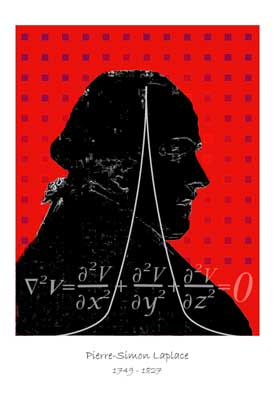
\includegraphics[scale=0.5]{images/LAPLACE.jpg}
  \end{columns}
}


\frame{{Derivation of L1}
  Substitute $F(t)=1$
  \begin{exampleblock}{L1}
    \begin{align*}
      F(p) &= \int_0^\infty 1\cdot d^{-pt}dt \\
      &= -\frac{1}{p}e^{-pt}\bigg\vert_0^\infty \\
      &= \frac{1}{p}
    \end{align*}
  \end{exampleblock}
  The real part of $p$ must be $>0$.
}


\frame{{The Magic Table}
  A table of Laplace transforms can be very handy.  One such table is available in Boas, pps 469 - 471.  A brief web search will turn up more, as well.  The tables contain transforms for both $f(t)$ and $F(p)$ and operate very much like the table for power series in Chapter 1 on page 26.
}


\frame{{Solutions of Differential Equations}
  Laplace transforms can be used to reduce ODEs to simpler algebraic equations.  We take the Laplace transform of each term in the differential equation.
  \begin{block}{$L(y')$}
    \begin{align*}
      L(y') &= \int_{0}^{\infty}y'(t)e^{-pt}dt \\
      &= e^{-pt}y(t)\bigg\vert_0^\infty -(-p)\int_{0}^{\infty}y(t)e^{-pt}dt \\
      &= pL(y) - y(0) \\
      &= pY-y_0
    \end{align*}
  \end{block}
}


\frame{{Solutions of Differential Equations (continued)}
  We continue for second order by re-writing $y''$ as $(y')'$
  \begin{block}{$L(y'')$}
    \begin{align*}
      L(y'') &= pL(y') - y'(0) \\
      &= p^2L(y) - py(0) - y'(0) \\
      &= p^2Y - py_0 - y'_0
    \end{align*}
  \end{block}
}


\frame{{Differential Equation Example}
  By using the table to look up the Laplace transforms we can find solutions to differential equations quite directly.  Using $L15$ and values $a=3$ and $p=2$ we directly calculate,
  \begin{exampleblock}{Example 5, page 442}
    \begin{align*}
      \int_{0}^{\infty}e^{-2t}\left( 1-\cos3t \right)dt &= \frac{3^2}{2\left( 2^2+3^2 \right)} \\
      &= \frac{9}{26}
    \end{align*}
  \end{exampleblock}
  We see that this is very powerful and convenient.
}

\frame{{Questions?}
	\begin{center}
		
\includegraphics[width=.7\textwidth]{images/fin.png}
	\end{center}
}

\end{document}
